\documentclass[a4paper,11pt]{article}
\input{/home/tof/Documents/Cozy/latex-include/preambule_doc.tex}
\input{/home/tof/Documents/Cozy/latex-include/preambule_commun.tex}
\newcommand{\showprof}{show them}  % comment this line if you don't want to see todo environment
\setlength{\fboxrule}{0.8pt}
\fancyhead[L]{\fbox{\Large{\textbf{Algo 08}}}}
\fancyhead[C]{\textbf{Exercices arbre binaire}}
\newdate{madate}{10}{09}{2020}
%\fancyhead[R]{\displaydate{madate}} %\today
\fancyhead[R]{Terminale - NSI}
\fancyfoot[L]{\vspace{1mm}Christophe Viroulaud}
\AtEndDocument{\label{lastpage}}
\fancyfoot[C]{\textbf{Page \thepage/\pageref{lastpage}}}
\fancyfoot[R]{\includegraphics[width=2cm,align=t]{/home/tof/Documents/Cozy/latex-include/cc.png}}

\begin{document}
\begin{exo}
    L'arbre figure \ref{arbre} représente une opération arithmétique.
    \begin{center}
        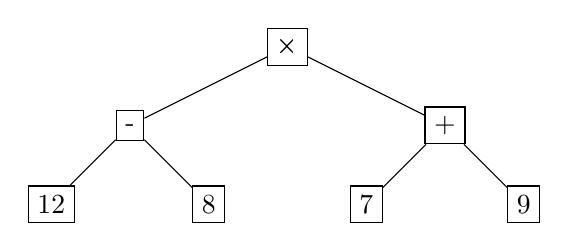
\begin{tikzpicture}
            \node[draw] (1) at (0,0) {×};
            \node[draw] (2) at (-2,-1) {-};
            \node[draw] (3) at (2,-1) {+};
            \node[draw] (4) at (-3,-2) {12};
            \node[draw] (5) at (-1,-2) {8};
            \node[draw] (6) at (1,-2) {7};
            \node[draw] (7) at (3,-2) {9};

            \draw (1) -- (2);
            \draw (1) -- (3);
            \draw (2) -- (4);
            \draw (2) -- (5);
            \draw (3) -- (6);
            \draw (3) -- (7);

        \end{tikzpicture}
        \captionof{figure}{Calcul arithmétique}
        \label{arbre}
    \end{center}
    \begin{enumerate}
        \item Parcourir cet arbre en profondeur (préfixe, infixe et postfixe).
        \item Donner le résultat du calcul.
        \item Pour quel parcours est-il indispensable de rajouter des parenthèses?
    \end{enumerate}
\end{exo}
\begin{exo}
    \begin{center}
    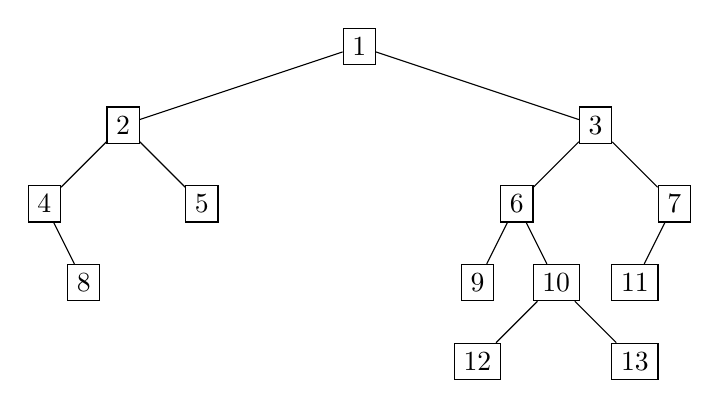
\begin{tikzpicture}
        \node[draw] (1) at (0,0) {1};
        \node[draw] (2) at (-3,-1) {2};
        \node[draw] (3) at (3,-1) {3};
        \node[draw] (4) at (-4,-2) {4};
        \node[draw] (5) at (-2,-2) {5};
        \node[draw] (6) at (2,-2) {6};
        \node[draw] (7) at (4,-2) {7};
        \node[draw] (8) at (-3.5,-3) {8};
        \node[draw] (9) at (1.5,-3) {9};
        \node[draw] (10) at (2.5,-3) {10};
        \node[draw] (11) at (3.5,-3) {11};
        \node[draw] (12) at (1.5,-4) {12};
        \node[draw] (13) at (3.5,-4) {13};

        \draw (1) -- (2);
        \draw (1) -- (3);
        \draw (2) -- (4);
        \draw (2) -- (5);
        \draw (3) -- (6);
        \draw (3) -- (7);
        \draw (4) -- (8);
        \draw (6) -- (9);
        \draw (6) -- (10);
        \draw (7) -- (11);
        \draw (10) -- (12);
        \draw (10) -- (13);
    \end{tikzpicture}
\end{center}

    \begin{enumerate}
        \item Effectuer les parcours (largeur, profondeur) sur l'arbre binaire.
        \item Quelle est la hauteur de cet arbre. On considère qu'un arbre vide à une hauteur de -1.
        \item Cet arbre est-il équilibré?
        \item Cet arbre est-il complet?
    \end{enumerate}
\end{exo}
\begin{exo}
    \begin{center}
        \begin{tikzpicture}
            \node[draw] (r) at (0,0) {r};
            \node[draw] (a) at (-3,-1) {a};
            \node[draw] (b) at (3,-1) {b};
            \node[draw] (c) at (-4,-2) {c};
            \node[draw] (d) at (-2,-2) {d};
            \node[draw] (e) at (2,-2) {e};
            \node[draw] (f) at (4,-2) {f};
            \node[draw] (g) at (-4.5,-3) {g};
            \node[draw] (h) at (-3.5,-3) {h};
            \node[draw] (i) at (-2.5,-3) {i};
            \node[draw] (j) at (-1.5,-3) {j};
            \node[draw] (k) at (1.5,-3) {k};
            \node[draw] (l) at (-2,-4) {l};

            \draw (r) -- (a);
            \draw (r) -- (b);
            \draw (a) -- (c);
            \draw (a) -- (d);
            \draw (b) -- (e);
            \draw (b) -- (f);
            \draw (c) -- (g);
            \draw (c) -- (h);
            \draw (d) -- (i);
            \draw (d) -- (j);
            \draw (e) -- (k);
            \draw (j) -- (l);
        \end{tikzpicture}
        \captionof{figure}{Un arbre de chaîne de caractère}
        \label{classebinaire}
    \end{center}
    L'objectif est de créer une classe permettant de construire un arbre binaire de chaînes de caractères \underline{distinctes}.
    \begin{enumerate}
        \item Créer la classe \textbf{\texttt{Arbre\_binaire}} et son constructeur. On passera un paramètre \textbf{\texttt{h}} qui initialisera l'attribut \texttt{\textbf{hauteur}} de l'arbre. Le constructeur initialisera:
              \begin{itemize}
                  \item un tableau \textbf{\texttt{arbre}} rempli d'objet \textbf{\texttt{None}} de la taille de l'arbre binaire parfait correspondant à \textbf{\texttt{h}}.
                  \item la racine de l'arbre avec la chaîne de caractère \textbf{\texttt{"r"}}.
              \end{itemize}
        \item Écrire la méthode \textbf{\texttt{get\_taille(self) $\rightarrow$ int}} qui renvoie le nombre de nœuds de l'arbre.
        \item Écrire la méthode \textbf{\texttt{get\_indice(self, chaine: str) $\rightarrow$ int}} qui renvoie la position de la chaîne dans le tableau.
        \item Écrire la méthode \textbf{\texttt{inserer(self, pere: str, gauche: str, droit: str) $\rightarrow$ None}} qui ajoute les fils \textbf{\texttt{gauche}} et \textbf{\texttt{droit}} au nœud \textbf{\texttt{pere}}.  La méthode lèvera une erreur d’assertion si le nœud \texttt{\textbf{pere}} ne peut pas avoir de fils (sort du tableau).
        \item Écrire la méthode récursive \textbf{\texttt{prefixe(self, position: int, parcours: list) $\rightarrow$ None}} qui effectue un parcours préfixe et complète le tableau \textbf{\texttt{parcours}} au fur et à mesure.
        \item Écrire sur le même modèle les méthodes \textbf{\texttt{infixe}} et \textbf{\texttt{postfixe}}
        \item \textbf{Pour les plus avancés:} Écrire la méthode récursive \textbf{\texttt{prefixe\_2(self, position: int) $\rightarrow$ list}} qui construit (par concaténation) le tableau de parcours.
    \end{enumerate}
\end{exo}
\end{document}